\documentclass[tikz,border=8pt]{standalone}
\usepackage[T1]{fontenc}
\usepackage{lmodern}
\usepackage{amsmath}
\usepackage{tikz}
\usetikzlibrary{arrows.meta,calc,fit,positioning,backgrounds}

\definecolor{ink}{HTML}{172033}
\definecolor{muted}{HTML}{61708A}
\definecolor{grid}{HTML}{D9E0EA}
\definecolor{panel}{HTML}{F7F9FC}
\definecolor{stagezero}{HTML}{2F80ED}
\definecolor{stagezerofill}{HTML}{EAF3FF}
\definecolor{stageone}{HTML}{E79A19}
\definecolor{stageonefill}{HTML}{FFF4DD}
\definecolor{fullbar}{HTML}{8E5CC7}
\definecolor{emptybar}{HTML}{168B6A}
\definecolor{danger}{HTML}{C94F5C}

\begin{document}
\sffamily
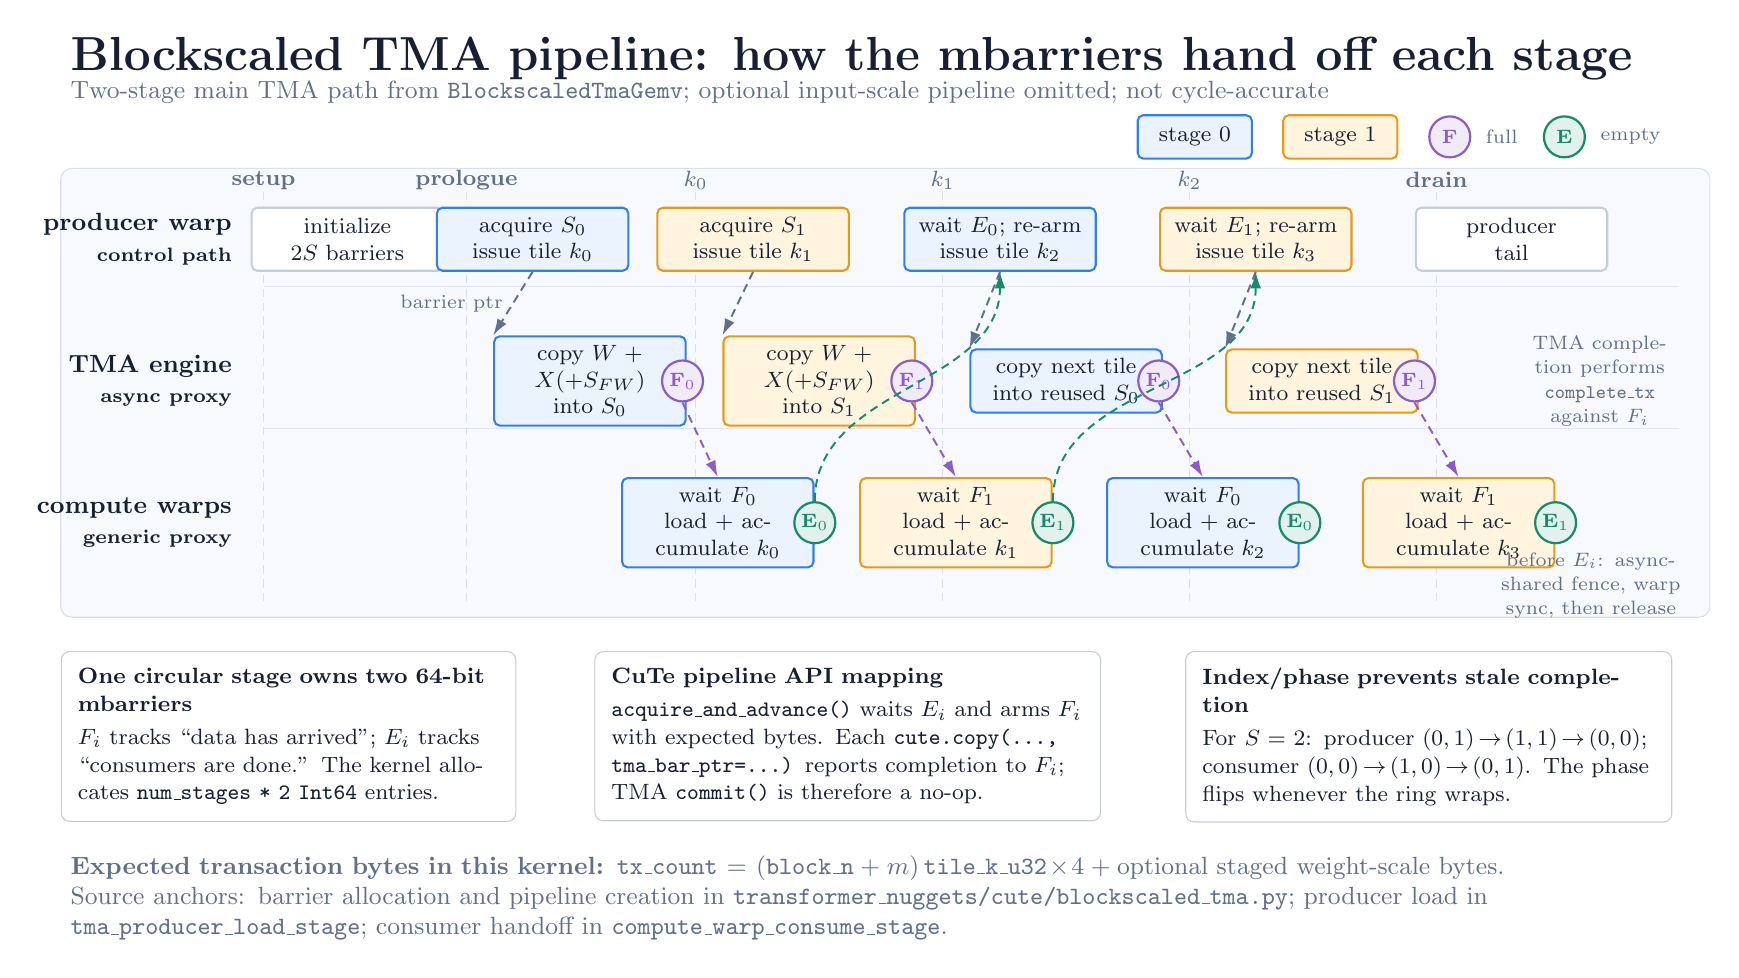
\begin{tikzpicture}[
  x=1.12cm,
  y=1cm,
  >={Latex[length=2.1mm,width=1.35mm]},
  title/.style={font=\bfseries\fontsize{17}{20}\selectfont, text=ink},
  subtitle/.style={font=\fontsize{9}{11}\selectfont, text=muted},
  lane label/.style={font=\bfseries\fontsize{9}{11}\selectfont, text=ink, align=right},
  tick/.style={font=\bfseries\fontsize{8}{10}\selectfont, text=muted},
  bar/.style={rounded corners=2pt, minimum height=8mm, text width=2.15cm, inner xsep=4pt,
              font=\fontsize{8}{9.5}\selectfont, align=center, line width=.75pt},
  s0/.style={bar, draw=stagezero, fill=stagezerofill, text=ink},
  s1/.style={bar, draw=stageone, fill=stageonefill, text=ink},
  neutral/.style={bar, draw=grid!90!ink, fill=white, text=ink},
  note/.style={draw=grid!90!ink, fill=white, rounded corners=3pt, inner sep=6pt,
               font=\fontsize{8}{10}\selectfont, text=ink, align=left},
  callout/.style={font=\fontsize{7.2}{8.8}\selectfont, text=muted, align=center},
  flow/.style={->, line width=.7pt, color=muted},
  dependency/.style={->, densely dashed, line width=.7pt, color=muted},
  full marker/.style={circle, draw=fullbar, fill=fullbar!12, line width=.8pt,
                      minimum size=5.2mm, inner sep=0pt,
                      font=\bfseries\fontsize{6.6}{7}\selectfont, text=fullbar},
  empty marker/.style={circle, draw=emptybar, fill=emptybar!12, line width=.8pt,
                       minimum size=5.2mm, inner sep=0pt,
                       font=\bfseries\fontsize{6.6}{7}\selectfont, text=emptybar},
]

% Header
\node[title, anchor=west] at (0,8.25) {Blockscaled TMA pipeline: how the mbarriers hand off each stage};
\node[subtitle, anchor=west] at (0,7.82)
  {Two-stage main TMA path from \texttt{BlockscaledTmaGemv}; optional input-scale pipeline omitted; not cycle-accurate};

% Legend
\node[s0, minimum width=1.45cm, minimum height=5.5mm, text width=1.15cm, anchor=west] at (12.2,7.25) {stage 0};
\node[s1, minimum width=1.45cm, minimum height=5.5mm, text width=1.15cm, anchor=west] at (13.85,7.25) {stage 1};
\node[full marker] (legend-full) at (15.75,7.25) {F};
\node[callout, anchor=west] at (16.05,7.25) {full};
\node[empty marker] (legend-empty) at (17.05,7.25) {E};
\node[callout, anchor=west] at (17.35,7.25) {empty};

% Timeline panel and lanes
\fill[panel, rounded corners=4pt] (0,1.15) rectangle (18.7,6.85);
\draw[grid, rounded corners=4pt] (0,1.15) rectangle (18.7,6.85);

\foreach \x/\label in {2.3/setup,4.6/prologue,7.2/$k_0$,10.0/$k_1$,12.8/$k_2$,15.6/drain} {
  \draw[grid, densely dashed] (\x,1.35) -- (\x,6.55);
  \node[tick] at (\x,6.7) {\label};
}

\node[lane label, anchor=east] at (2.05,5.95) {producer warp\\\scriptsize control path};
\node[lane label, anchor=east] at (2.05,4.15) {TMA engine\\\scriptsize async proxy};
\node[lane label, anchor=east] at (2.05,2.35) {compute warps\\\scriptsize generic proxy};

\draw[grid!80] (2.3,5.35) -- (18.35,5.35);
\draw[grid!80] (2.3,3.55) -- (18.35,3.55);

% Producer lane
\node[neutral, minimum width=1.75cm] (init) at (3.25,5.95)
  {initialize\\$2S$ barriers};
\node[s0, minimum width=2.05cm] (p0) at (5.35,5.95)
  {acquire $S_0$\\issue tile $k_0$};
\node[s1, minimum width=2.15cm] (p1) at (7.85,5.95)
  {acquire $S_1$\\issue tile $k_1$};
\node[s0, minimum width=2.3cm] (p2) at (10.65,5.95)
  {wait $E_0$; re-arm\\issue tile $k_2$};
\node[s1, minimum width=2.3cm] (p3) at (13.55,5.95)
  {wait $E_1$; re-arm\\issue tile $k_3$};
\node[neutral, minimum width=1.55cm] (tail) at (16.45,5.95)
  {producer\\tail};

% TMA lane
\node[s0, minimum width=2.25cm] (t0) at (6.0,4.15)
  {copy $W+X(+S_{FW})$\\into $S_0$};
\node[s1, minimum width=2.25cm] (t1) at (8.6,4.15)
  {copy $W+X(+S_{FW})$\\into $S_1$};
\node[s0, minimum width=2.25cm] (t2) at (11.4,4.15)
  {copy next tile\\into reused $S_0$};
\node[s1, minimum width=2.25cm] (t3) at (14.3,4.15)
  {copy next tile\\into reused $S_1$};

\node[full marker] (f0a) at (7.05,4.15) {F$_0$};
\node[full marker] (f1a) at (9.65,4.15) {F$_1$};
\node[full marker] (f0b) at (12.45,4.15) {F$_0$};
\node[full marker] (f1b) at (15.35,4.15) {F$_1$};

% Consumer lane
\node[s0, minimum width=2.35cm] (c0) at (7.45,2.35)
  {wait $F_0$\\load + accumulate $k_0$};
\node[s1, minimum width=2.35cm] (c1) at (10.15,2.35)
  {wait $F_1$\\load + accumulate $k_1$};
\node[s0, minimum width=2.35cm] (c2) at (12.95,2.35)
  {wait $F_0$\\load + accumulate $k_2$};
\node[s1, minimum width=2.35cm] (c3) at (15.85,2.35)
  {wait $F_1$\\load + accumulate $k_3$};

\node[empty marker] (e0a) at (8.55,2.35) {E$_0$};
\node[empty marker] (e1a) at (11.25,2.35) {E$_1$};
\node[empty marker] (e0b) at (14.05,2.35) {E$_0$};
\node[empty marker] (e1b) at (16.95,2.35) {E$_1$};

% Issue/completion/reuse dependencies
\draw[dependency] (p0.south) -- node[callout, left] {barrier ptr} (t0.north west);
\draw[dependency] (p1.south) -- (t1.north west);
\draw[dependency] (p2.south) -- (t2.north west);
\draw[dependency] (p3.south) -- (t3.north west);

\draw[dependency, color=fullbar] (f0a.south) -- (c0.north);
\draw[dependency, color=fullbar] (f1a.south) -- (c1.north);
\draw[dependency, color=fullbar] (f0b.south) -- (c2.north);
\draw[dependency, color=fullbar] (f1b.south) -- (c3.north);

\draw[dependency, color=emptybar] (e0a.north) to[out=90,in=-90] (p2.south);
\draw[dependency, color=emptybar] (e1a.north) to[out=90,in=-90] (p3.south);

\node[callout, text width=2.4cm] at (17.45,4.15)
  {TMA completion performs\\\texttt{complete\_tx} against $F_i$};
\node[callout, text width=2.6cm] at (17.35,1.55)
  {before $E_i$: async-shared fence, warp sync, then release};

% Lower explanatory panels
\node[note, anchor=north west, text width=5.35cm] (contract) at (0,0.72) {
  \textbf{One circular stage owns two 64-bit mbarriers}\\[2pt]
  $F_i$ tracks ``data has arrived''; $E_i$ tracks ``consumers are done.''
  The kernel allocates \texttt{num\_stages * 2} \texttt{Int64} entries.
};

\node[note, anchor=north west, text width=6.0cm] (api) at (6.05,0.72) {
  \textbf{CuTe pipeline API mapping}\\[2pt]
  \texttt{acquire\_and\_advance()} waits $E_i$ and arms $F_i$ with expected bytes.
  Each \texttt{cute.copy(..., tma\_bar\_ptr=...)} reports completion to $F_i$;
  TMA \texttt{commit()} is therefore a no-op.
};

\node[note, anchor=north west, text width=5.75cm] (phase) at (12.75,0.72) {
  \textbf{Index/phase prevents stale completion}\\[2pt]
  For $S=2$: producer $(0,1)\!\to\!(1,1)\!\to\!(0,0)$; consumer
  $(0,0)\!\to\!(1,0)\!\to\!(0,1)$. The phase flips whenever the ring wraps.
};

% Footer formula and source mapping
\node[subtitle, anchor=north west, text width=18.4cm] at (0,-1.75) {
  \textbf{Expected transaction bytes in this kernel:}
  $\texttt{tx\_count}=(\texttt{block\_n}+m)\,\texttt{tile\_k\_u32}\!\times\!4
  + \text{optional staged weight-scale bytes}$.
  Source anchors: barrier allocation and pipeline creation in
  \texttt{transformer\_nuggets/cute/blockscaled\_tma.py}; producer load in
  \texttt{tma\_producer\_load\_stage}; consumer handoff in
  \texttt{compute\_warp\_consume\_stage}.
};

\end{tikzpicture}
\end{document}
